\documentclass[12pt, a4paper]{ctexart}

% --- 宏包引入 ---
\usepackage[utf8]{inputenc}
\usepackage{geometry}
\geometry{left=2.5cm, right=2.5cm, top=3cm, bottom=3cm}
\usepackage{amsmath, amssymb}
\usepackage{graphicx}
\usepackage{fancyhdr}
\usepackage{hyperref}
\usepackage{setspace}
\usepackage{booktabs} % 用于表格
\usepackage{caption}
\usepackage{enumitem}
\usepackage{tabularx}
\usepackage{booktabs}
\usepackage{fontawesome5}
\usepackage{float}

% --- 样式设置 ---
\hypersetup{
    colorlinks=true,
    linkcolor=black,
    filecolor=blue,      
    urlcolor=blue,
    citecolor=black,
}

% 设置页眉页脚 (仿照 Report.pdf)
\pagestyle{fancy}
\fancyhf{}
\fancyhead[L]{Rust程序设计}
\fancyhead[R]{2026 Spring}
\fancyfoot[C]{\thepage}
\renewcommand{\headrulewidth}{0.4pt}

% 设置行间距
\linespread{1.5}

% --- 文档开始 ---
\begin{document}

% --- 封面 (仿照 Report.pdf 布局) ---
\begin{titlepage}
    \centering
    \vspace*{2cm}
    {\Huge \bfseries Rust程序设计课程项目报告 \par}
    \vspace{1cm}
    {\Large \bfseries Mini-Lisp 解释器实现 \par}
    
    \vspace{3cm}
    
    \begin{spacing}{1.5}
    \large
    \begin{tabular}{llc}
        成员: & 周静怡 & 2400013056 \\
              & 王嘉怡 & 2400013107 \\
    \end{tabular}
    \end{spacing}

    \vfill
    {\large Rust程序设计 (春季, 2026) \par}
    {\large 北京大学 \par}
    {\large 2026年6月29日 \par}
\end{titlepage}

% --- 目录 ---
\newpage
\tableofcontents
\newpage

% --- 正文内容 ---
\section*{MiniLisp-RS 项目}
\addcontentsline{toc}{section}{MiniLisp-RS 项目}

\section*{1. 项目概述}
\addcontentsline{toc}{section}{1. 项目概述}

Mini-Lisp 是对 Lisp 语言的一种简化实现形式，保留了 S 表达式、符号求值、函数式调用、闭包和列表处理等核心特征。本项目以 Rust 为实现语言，完成了一个轻量级 Mini-Lisp 解释器，并在命令行解释执行的基础上扩展了图形界面。

我们曾在软件设计实践课程中，使用C++实现了一个类似的 Mini-Lisp 解释器，在当时体验到了大量的面向对象编程的思想。因此，我们产生了用 Rust 实现一个新版本的想法，期望借此更深刻地体会 Rust 语言的不同特性。

故而，本项目的主要目标包括三个方面：第一，实现一个能够正确解析并求值 Mini-Lisp 表达式的解释器，支持基本算术、条件判断、变量定义、匿名函数、列表操作和若干内置过程。第二，在此前使用 C++ 实现类似解释器的经验基础上，尝试使用 Rust 重新设计该项目，从而体会 Rust 在所有权、模式匹配、错误处理和模块化组织方面的特点。第三，我们希望在解释器核心之外提供更友好的使用方式，即完成解释器的桌面图形界面。

从最终结果来看，项目已经形成了较完整的系统：既可以通过 REPL 逐行输入 Lisp 表达式，也可以直接执行 \verb|.scm| 文件；图形界面支持输入区、输出区、按钮控制、语法高亮以及括号匹配提示等功能，使得 Mini-Lisp 的演示和调试更直观。

\section*{2. 项目文件结构}
\addcontentsline{toc}{section}{2. 项目文件结构}

项目的核心语言逻辑位于 \verb|src/| 目录下，图形界面入口位于 \verb|src/bin/| 下。其主要文件结构如下：

\begin{verbatim}
src/
├── lib.rs             对外库入口，提供统一执行接口
├── main.rs            命令行入口，负责 REPL 与文件执行
├── token.rs           Token 定义
├── tokenizer.rs       词法分析器
├── parser.rs          语法分析器
├── value.rs           运行时值的表示
├── eval_env.rs        求值环境与求值器
├── form.rs            特殊形式实现
├── builtins.rs        内置过程实现
├── output.rs          输出抽象
└── error.rs           错误类型定义和错误打印

src/bin/
└── gui.rs             GUI 程序入口

src/bin/gui/
├── theme.rs           GUI 主题、颜色、字号、尺寸配置
└── editor.rs          编辑器高亮与装饰逻辑
\end{verbatim}

\section*{3. 使用方法与可用功能}
\addcontentsline{toc}{section}{3. 使用方法与可用功能}

\subsection*{3.1 命令行使用方式}
\addcontentsline{toc}{subsection}{3.1 命令行使用方式}

项目支持以命令行形式启动交互式 REPL：

\begin{verbatim}
cargo run --bin mini_lisp_rs
\end{verbatim}

按 Ctrl+Z 退出。

也支持直接执行一个 Lisp 源文件：

\begin{verbatim}
cargo run --bin mini_lisp_rs sort_test1.scm
\end{verbatim}

(sort\_test1.scm是我们提供的排序算法示例文件)

在命令行模式下，用户可以逐条输入表达式并立即查看求值结果，这对于调试解释器行为、验证内置函数和测试递归过程都很方便。

\subsection*{3.2 图形界面使用方式}
\addcontentsline{toc}{subsection}{3.2 图形界面使用方式}

除了命令行模式外，项目还实现了一个独立的桌面图形界面：

\begin{verbatim}
cargo run --release --bin gui
\end{verbatim}

构建完成后，也可以直接点击运行生成的可执行文件，不再依赖 PowerShell：

\begin{verbatim}
target/release/gui.exe
\end{verbatim}

这一点提升了项目的可用性和演示效果。

\subsection*{3.3 当前支持的语言功能}
\addcontentsline{toc}{subsection}{3.3 当前支持的语言功能}

目前解释器已经支持以下功能：

\begin{itemize}
\item 数值与布尔值的表示和运算
\item 符号求值与变量绑定
\item \verb|define|、\verb|lambda|、\verb|if|、\verb|begin|、\verb|cond|、\verb|let| 等特殊形式
\item 列表、序对以及基础列表处理过程
\item \verb|car|、\verb|cdr|、\verb|cons|、\verb|append| 等基础内置过程
\item \verb|map|、\verb|filter|、\verb|reduce| 等高阶函数
\item 文件输入与批量执行
\end{itemize}

\subsection*{3.4 图形界面的辅助功能}
\addcontentsline{toc}{subsection}{3.4 图形界面的辅助功能}

在图形界面部分，项目实现了以下提升体验的编辑器功能：

\begin{itemize}
\item 输入框和输出框左右分栏显示，便于对照查看
\item 一键执行(Run)、清空输出(Clear Output)、重置环境(Reset Env)
\item 查看示例代码和已实现的语言功能（包括特殊形式(Special Forms)和内置过程(Built-in Procedures)）的按钮(Reference)
\item 输入文本的自动语法着色
\item 括号匹配提示
\end{itemize}

\section*{4. 系统设计与实现细节}
\addcontentsline{toc}{section}{4. 系统设计与实现细节}

\subsection*{4.1 总体设计思路}
\addcontentsline{toc}{subsection}{4.1 总体设计思路}

系统整体采用分层设计。最底层是词法分析与语法分析，中间层是运行时值表示、求值环境和表达式求值逻辑，最上层是命令行与图形界面两种输入输出前端。用户输入一段 Lisp 代码后，系统首先将源码拆分为 token，再将 token 解析为内部表达式结构，最后在求值环境中执行并返回结果。

\subsection*{4.2 解释器核心模块实现}
\addcontentsline{toc}{subsection}{4.2 解释器核心模块实现}

\paragraph*{词法分析模块}


词法分析器 tokenizer 负责将用户输入的字符串拆分成一系列 token。

例如，对于输入：

\begin{verbatim}
(+ 1 2)
\end{verbatim}

词法分析器会将其转换为：

\begin{verbatim}
LeftParen, Identifier("+"), Number(1), Number(2), RightParen
\end{verbatim}

该模块主要处理括号、数字、字符串、布尔值和标识符等基本词法单元。

\paragraph*{语法分析模块}
语法分析器 parser 负责根据 token 序列构造 Mini-Lisp 表达式。由于 Lisp 的语法结构非常统一，主要由原子表达式和列表表达式组成，因此语法分析的核心是递归处理括号嵌套结构。

例如：

\begin{verbatim}
(+ 1 (* 2 3))
\end{verbatim}

会被解析为一个嵌套表达式，其中外层表达式表示 \verb|+| 函数调用，内层表达式表示 \verb|*| 函数调用。

\paragraph*{运行时值表示}
本项目使用 \verb|enum| 表示不同类型的运行时值，例如 \verb|Numeric|、\verb|Boolean|、\verb|Pair| 等，并通过 \verb|match| 对不同情况进行处理。

\paragraph*{求值环境}
求值环境用于保存变量名到值的绑定关系。例如执行：

\begin{verbatim}
(define x 10)
\end{verbatim}

之后，环境中会记录 \verb|x| 对应的值为 \verb|10|。当之后输入：

\begin{verbatim}
(+ x 5)
\end{verbatim}

解释器会先在环境中查找 \verb|x|，再进行求值。项目中，环境不仅负责保存当前作用域内的变量绑定，还通过父环境指针形成链式作用域结构，从而支持一些函数变量的局部作用域需求。相关逻辑主要由 \verb|eval_env.rs| 管理。

\paragraph*{表达式求值}
求值器是解释器的核心模块。它根据表达式的不同形式执行不同逻辑：

\begin{itemize}
\item 如果表达式是数字、布尔值或字符串，则直接返回自身。
\item 如果表达式是符号，则在环境中查找其绑定值。
\item 如果表达式是列表，则将其视为特殊形式或函数调用。
\item 如果表达式不合法，则返回相应错误。
\end{itemize}

\paragraph*{特殊形式与内置过程}
在 Lisp 中，并不是所有表达式都遵循统一规则，例如 \verb|define|、\verb|if|、\verb|lambda|、\verb|begin|、\verb|cond| 和 \verb|let| 都具有自己的求值语义。因此，我们将这类语法结构单独放入 \verb|form.rs| 中实现，以便与普通函数调用区分开来。

我们在 \verb|builtins.rs| 中集中实现具体内置过程的逻辑，主要包括算术运算、比较运算、列表操作以及若干高阶函数。

\section*{5. Rust 使用特点与 C++ 对比分析}
\addcontentsline{toc}{section}{5. Rust 使用特点与 C++ 对比分析}

在项目中，我们也切身体会到了Rust与C++编程语言风格的不同。

比如最开始做C++版本时，我们使用大量的面向对象设计模式，将Value作为抽象基类，再派生出数值、字符串、布尔等不同子类，每个子类都有自己的实现。而在Rust版本中，我们使用枚举来表示不同类型的值，每个枚举变体对应一种类型的值，通过 \verb|match| 对不同情况进行处理。对于其他类似面向对象中“共享行为”的需求，在rust中也会使用\verb|struct| 加上 \verb|trait| 的方式实现。在当前的解释器代码编写体验里，Rust版本似乎是更舒适一些的。

在原本的C++ 实现中，我们大量使用 \verb|std::shared_ptr| 管理值对象和环境对象，以便在表达式、环境链和闭包之间共享数据。这是更加方便的，但需要程序员自行维护何时访问何时修改的问题。Rust 实现虽然同样使用引用计数，但会把共享和修改区分开。对于运行时值，我们使用 Rc<Value> 可共享；而对于求值环境，我们使用 Rc<RefCell<EvalEnv>>，表示被共同持有的同时还需被修改。但这样做的代码复杂度也大大增加了。

在错误处理时，C++ 版本里若使用异常，错误传播路径有时不那么直观；如果不用异常，又容易变成手动检查返回值，比较麻烦。Rust 里的 \verb|Result<T, E>| 机制要求错误处理直接体现在函数签名中。本项目中的求值也大量采用 \verb|Result<ValuePtr, LispError>| 返回值，使语法错误、运行时错误以及类似退出解释器这样的控制流都能够在类型层面被统一描述。

\section*{6. 结果展示}
\addcontentsline{toc}{section}{6. 结果展示}

本项目已经能够支持 Mini-Lisp 的基本解释执行，并提供命令行与图形界面两种交互模式。

以下为项目运行截图展示：

\begin{figure}[H]
    \centering
    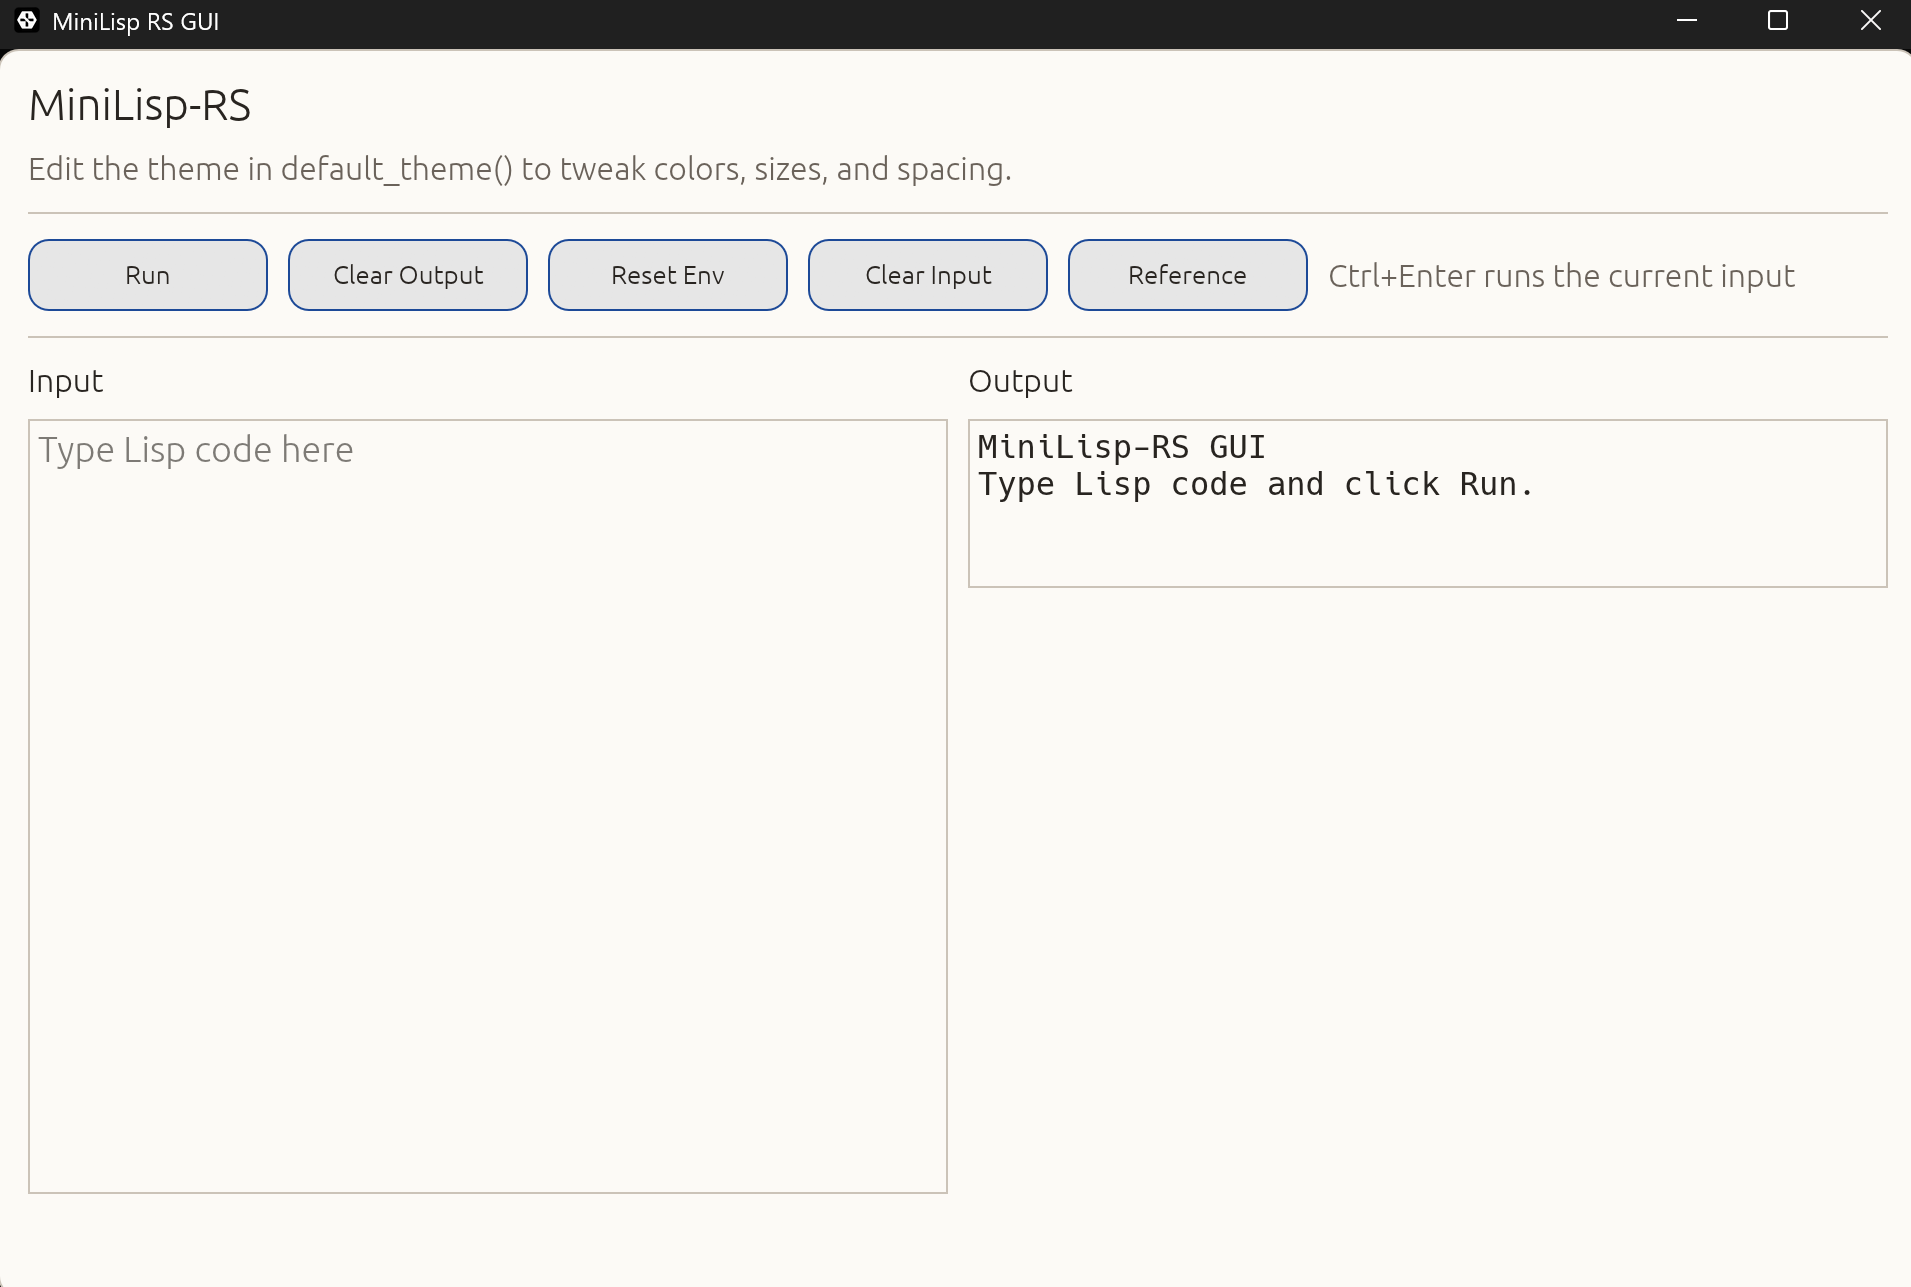
\includegraphics[width=0.75\textwidth]{gui_start.png}
    \caption{初始界面展示}
\end{figure}

\begin{figure}[H]
    \centering
    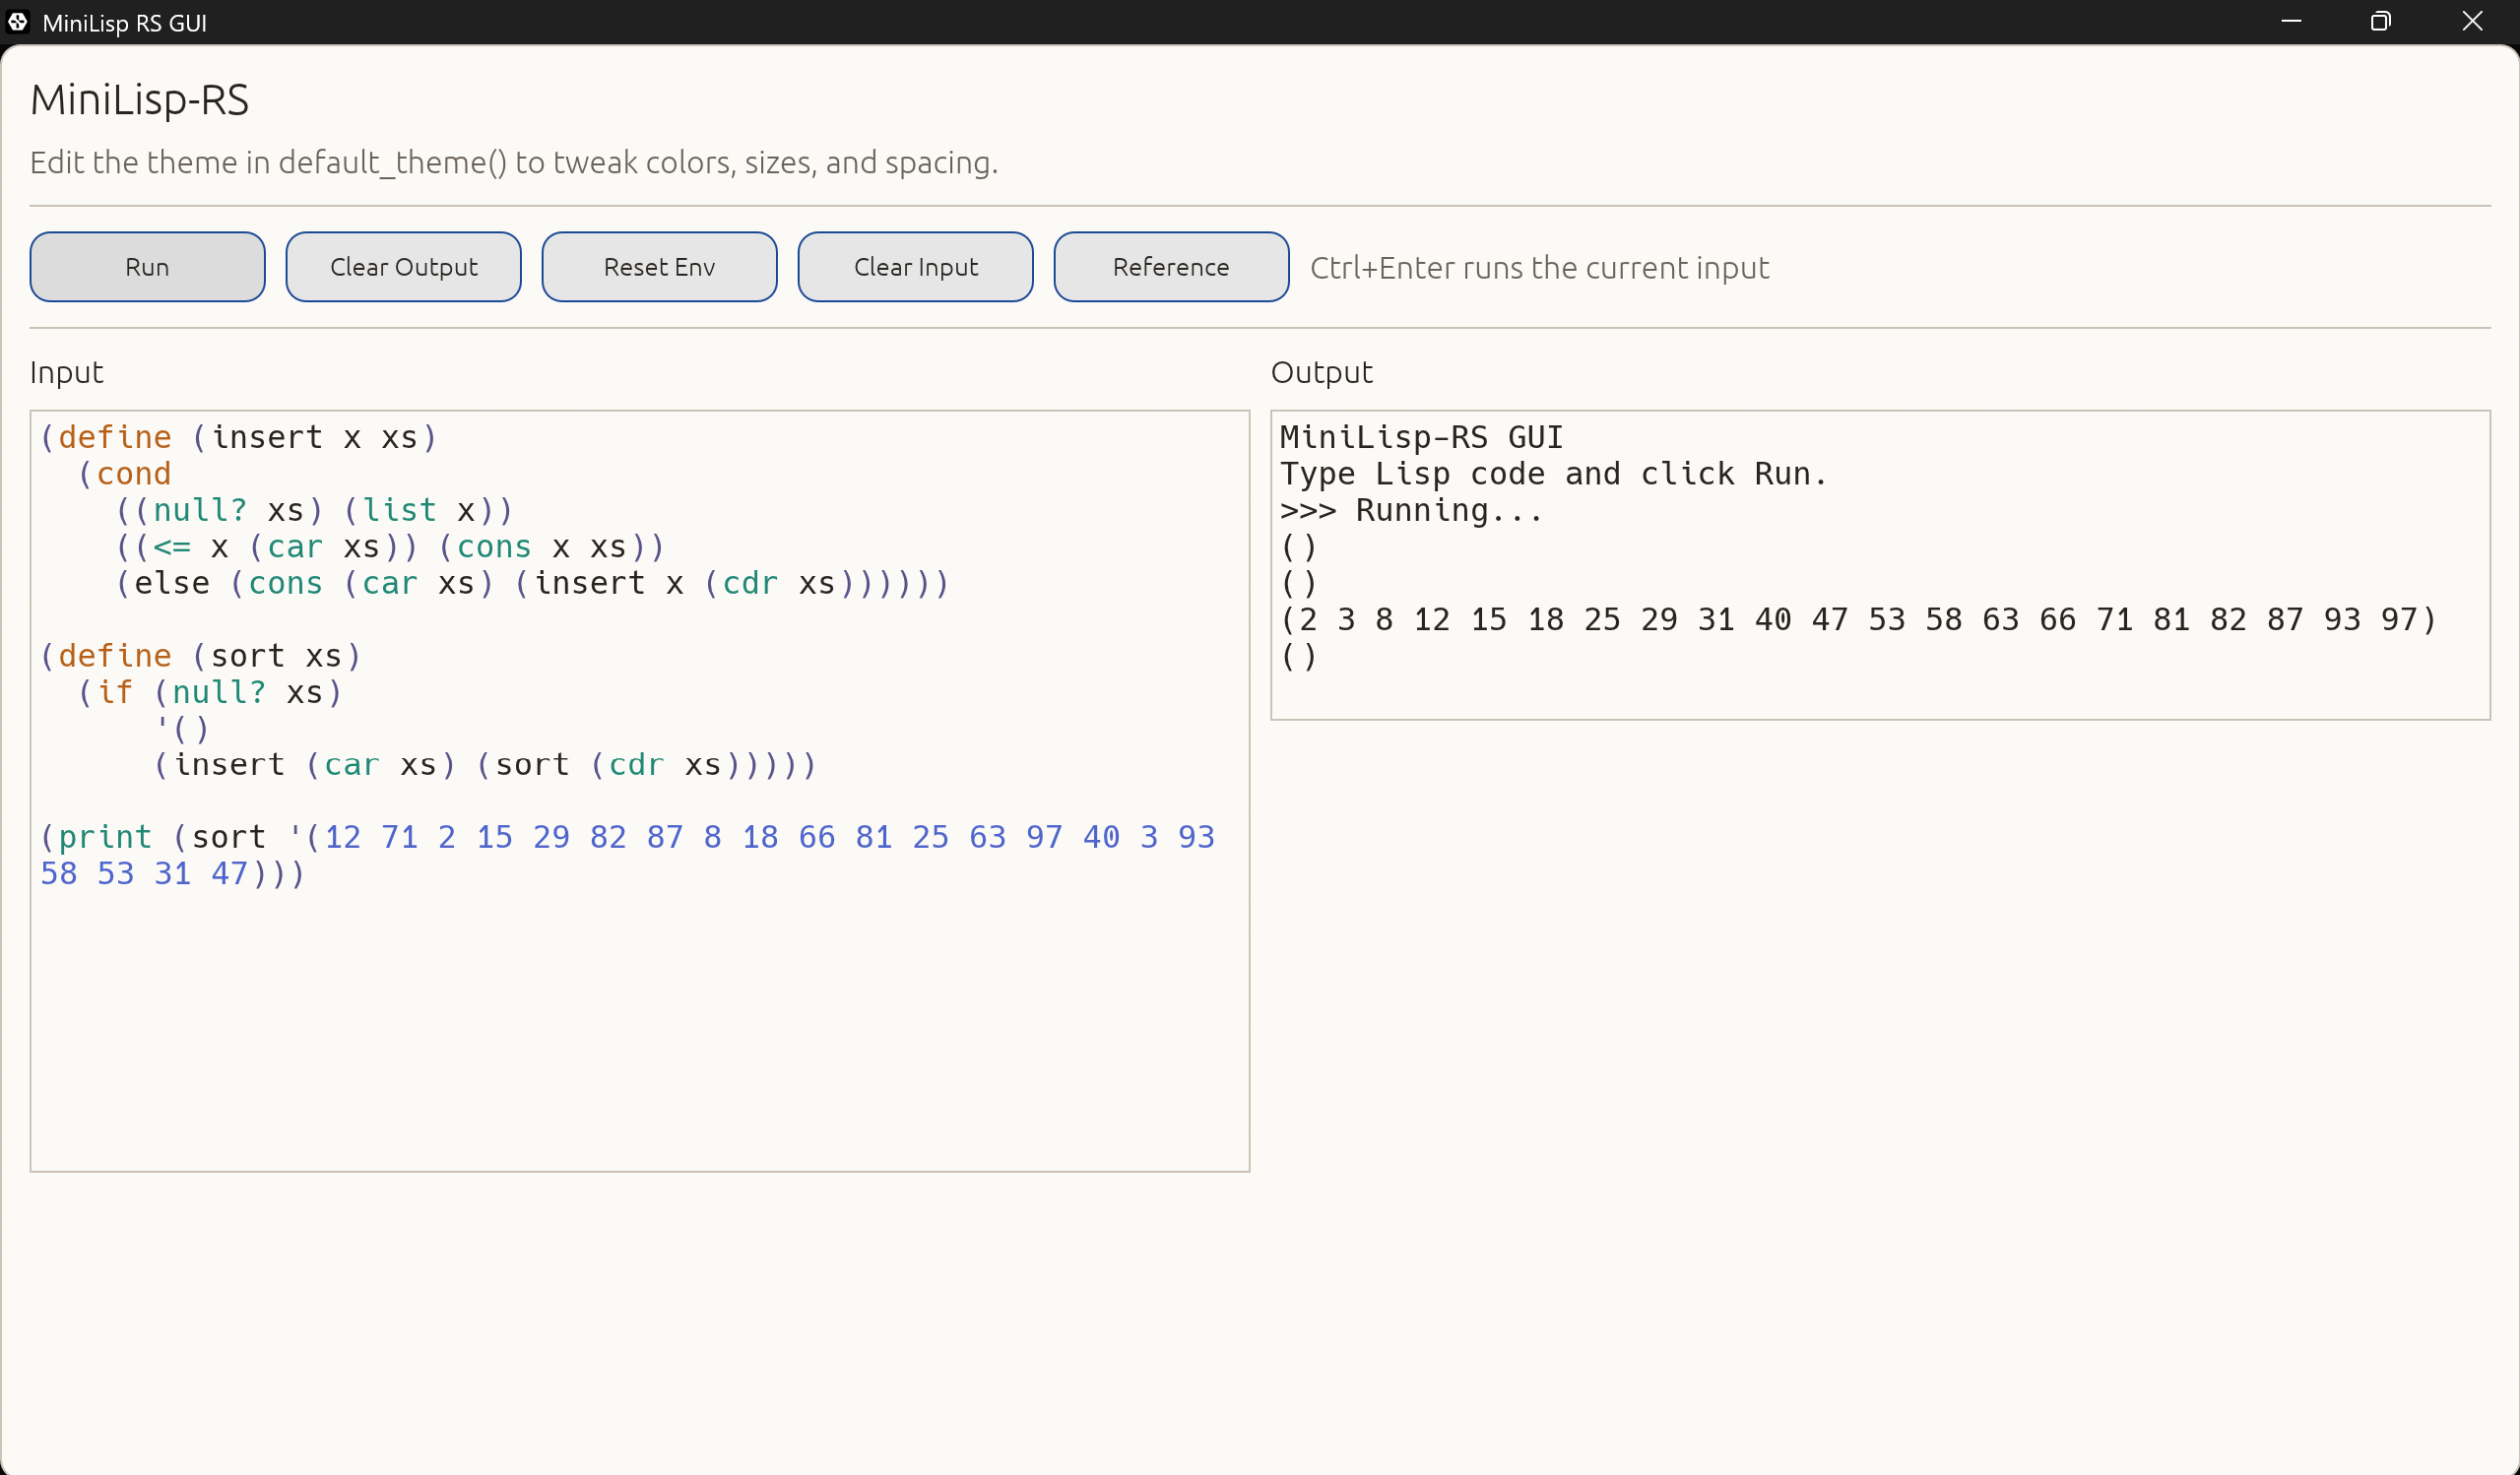
\includegraphics[width=0.85\textwidth]{gui_run.png}
    \caption{运行效果展示}
\end{figure}

\begin{figure}[H]
    \centering
    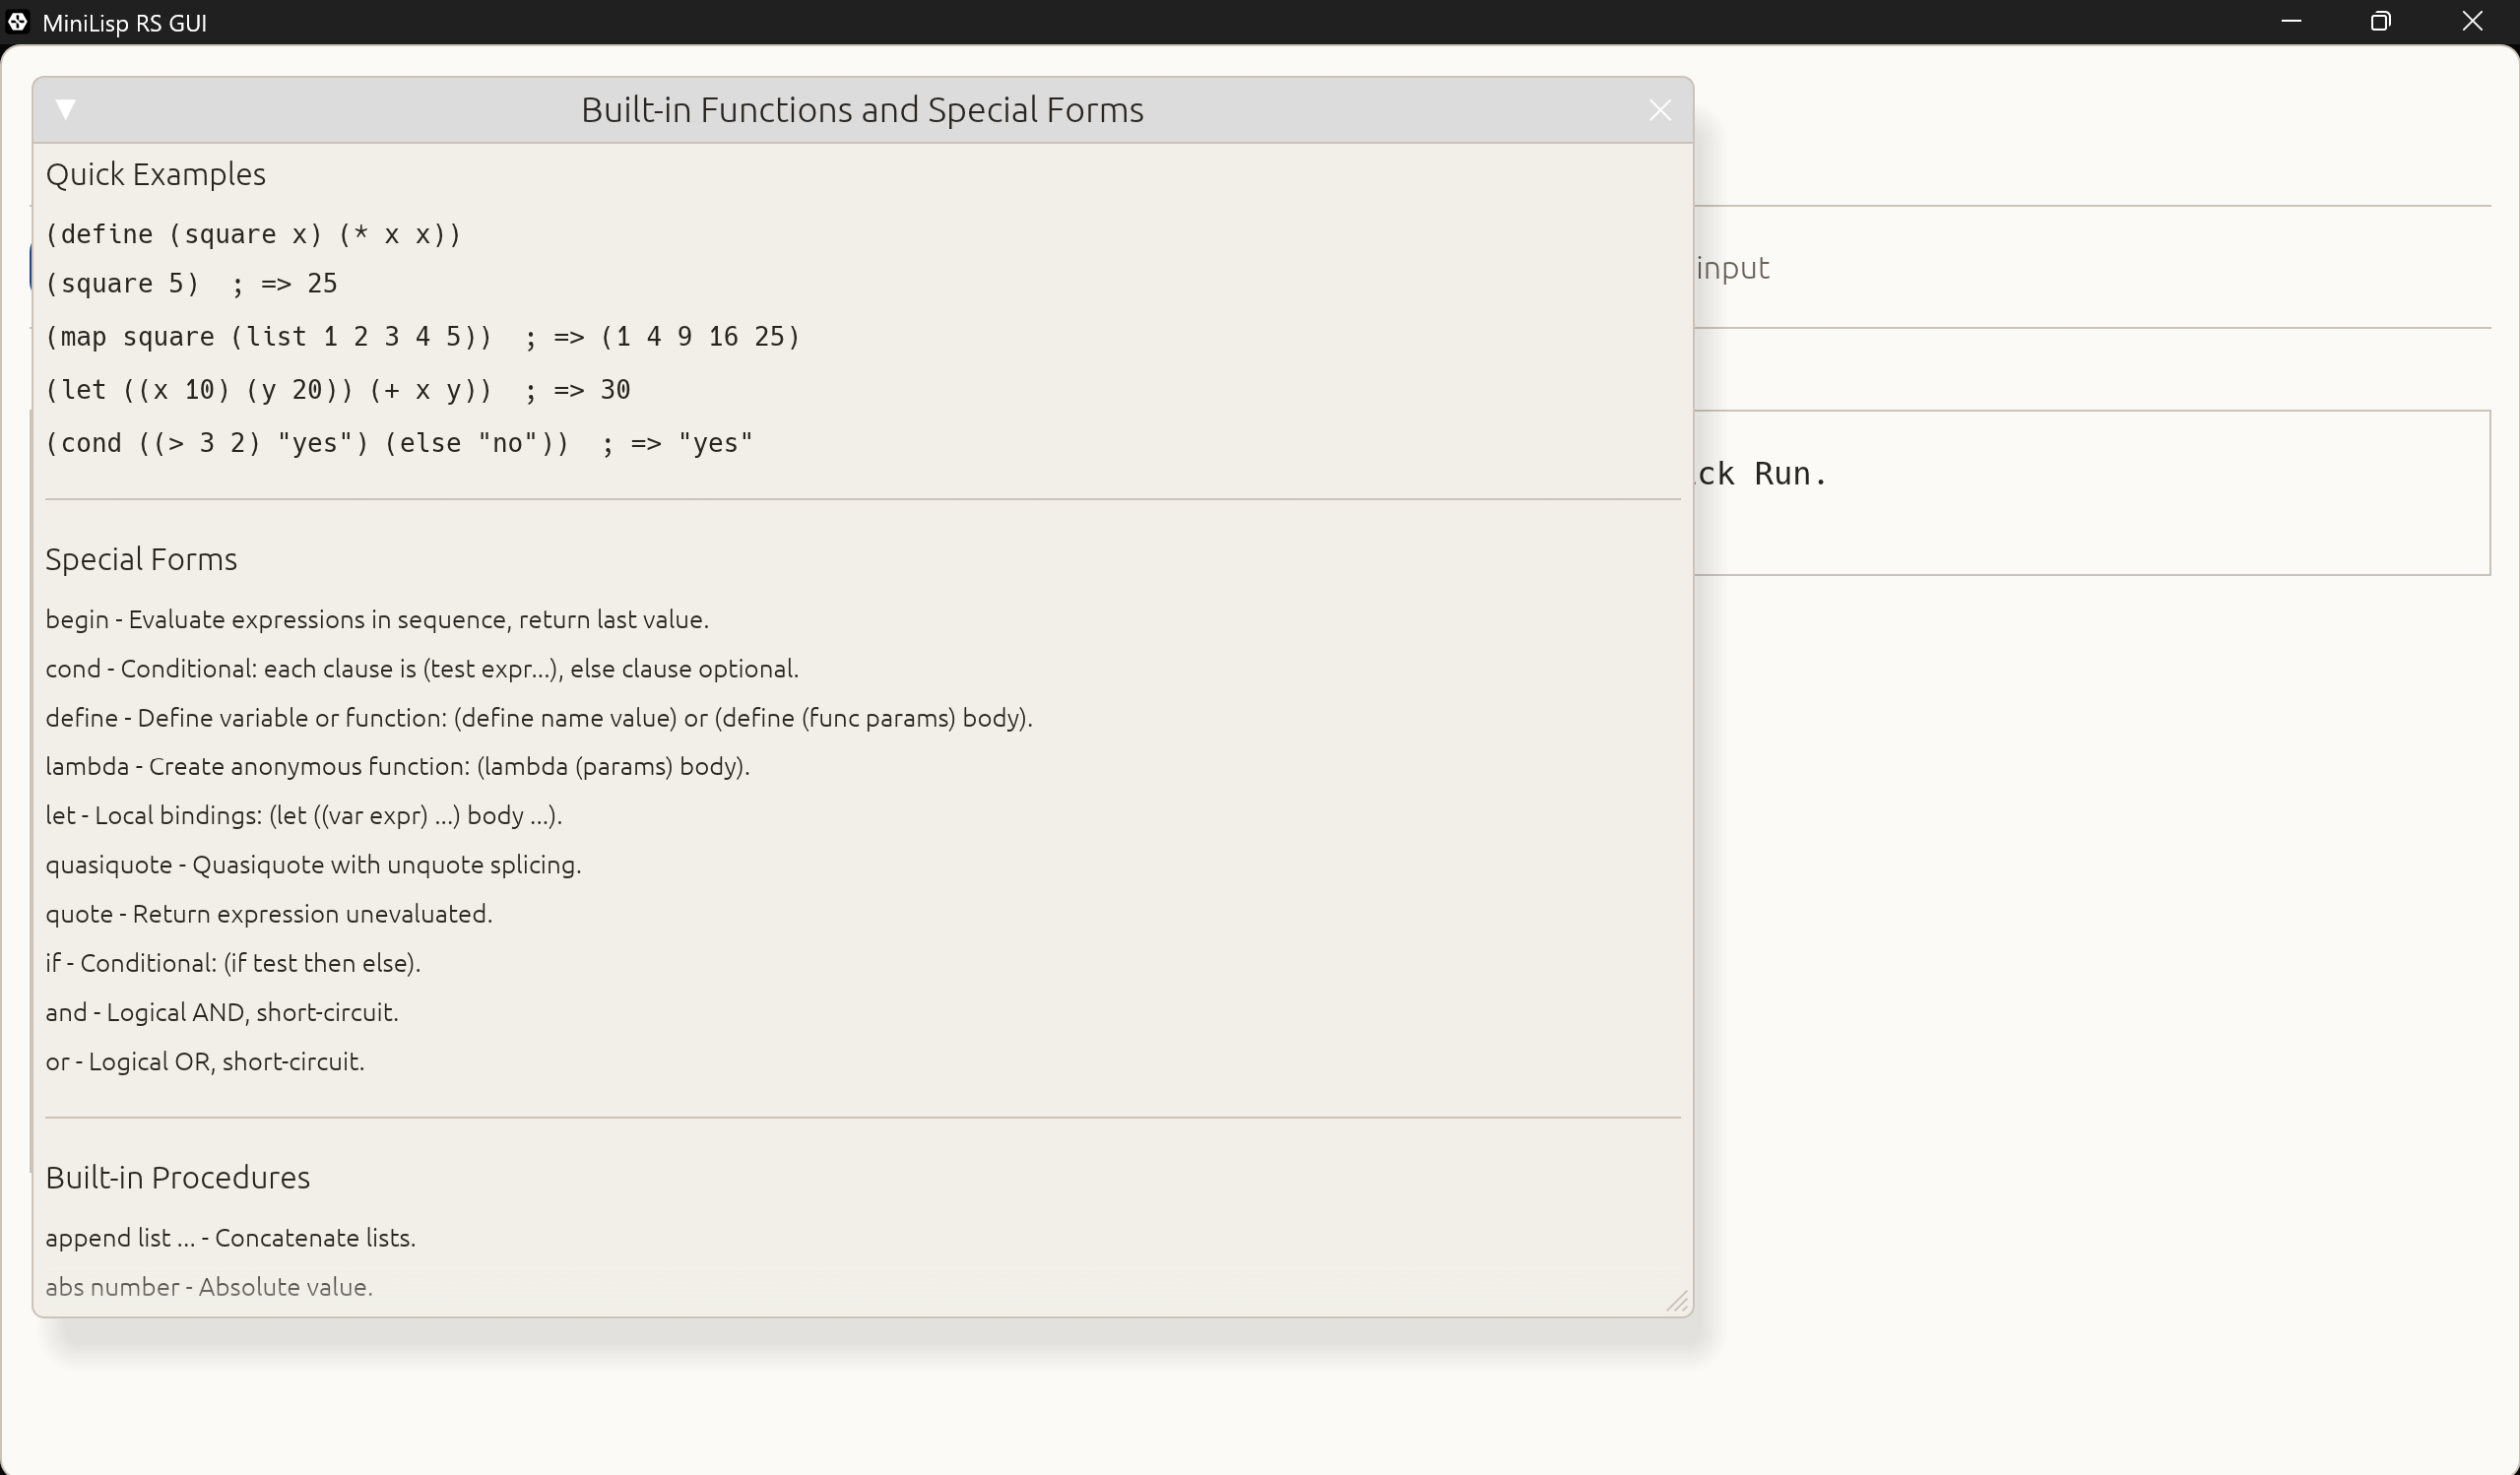
\includegraphics[width=0.85\textwidth]{gui_reference.png}
    \caption{教程文档功能展示}
\end{figure}

\section*{7. 总结}
\addcontentsline{toc}{section}{7. 总结}

\subsection*{7.1 项目亮点与不足}
\addcontentsline{toc}{subsection}{7.1 项目亮点与不足}

本项目的主要亮点在于：

\begin{itemize}
\item 较完整地实现了一个 Mini-Lisp 解释器，覆盖了解析、求值、闭包、特殊表单和高阶函数等关键内容。
\item 解释器核心之外实现了独立桌面 GUI，提供较好的使用体验和可视化结果。
\item 在实现过程中体现了 Rust 与 C++ 不同的工程思维方式，为后续语言实现学习提供了比较样本。
\end{itemize}

当然，项目仍有进一步完善空间：

\begin{itemize}
\item 目前 GUI 仍以轻量级编辑器体验为主，尚未加入更复杂的调试辅助能力。
\item 解释器支持的语言特性也仍然是 Mini-Lisp 级别，没有涉及宏系统以及更完整的标准库。
\end{itemize}

\subsection*{7.2 分工说明}
\addcontentsline{toc}{subsection}{7.2 分工说明}

本次项目的分工如下：

\begin{itemize}
\item 周静怡：负责项目初始框架搭建，完成早期词法分析器、语法分析框架的建立；参与后续解释器功能扩展，包括 \verb|lambda| 求值等部分特殊形式，以及添加具体内置过程；完善文件输入功能；完成 GUI 界面实现，加入自动着色等功能；报告撰写。
\item 王嘉怡：负责语法分析器的完善与接口调整，完成解释器求值、变量定义与查找、调用内置过程等功能；进行解释器调试测试与 bug 修复；完成 GUI 功能优化，包括输入清除、示例代码和语言规则查看功能。
\end{itemize}

本项目的全部代码可见https://github.com/Janezzzhou/MiniLisp-RS

\end{document}
